\documentclass[11pt]{article}
\usepackage{geometry}
\usepackage{amsmath}
\usepackage{amssymb}
\usepackage{enumitem}
\usepackage{fancyhdr}
\usepackage{tikz}
\usepackage{tcolorbox}

\usetikzlibrary{trees}
\pagestyle{fancy}

\lhead{MTH 201 (Calculus)}
\chead{Activities: Extended Chain Rule practice}
\rhead{2018-10-10}

\begin{document}

\noindent
This activity will challenge you to apply the Chain Rule in situations where we have incomplete information about the functions involved, or where the functions involved are given as graphs or tables rather than formulas. 

\subsection*{Warmup}

Let $f$ and $g$ be differentiable functions and $y = f(g(x))$. Then the Chain Rule says that the derivative $y'$ is...

$$y' = \hspace{3in}$$

\subsection*{Chain Rule with partial information}

Suppose $f$ and $g$ are functions and the only thing we know about them is the following: 
$$f(2) = 10 \qquad g(2) = -3  \qquad f'(-3) = -2 \qquad g'(2) = 4$$
Also let $A(x) = f(g(x))$. Question: Is it possible with just this information to find the value of $A'(2)$? If so, find it. If not, explain exactly what piece(s) of information you would need to find $A'(2).$

\subsection*{Chain Rule with graphs}

Let $f$ and $g$ be given by the graphs: 

\begin{center}
    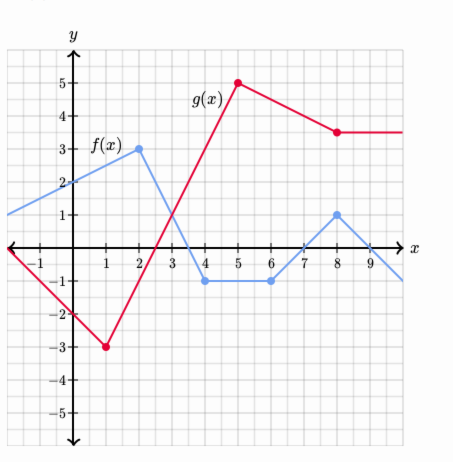
\includegraphics[width=3in]{Chainrule-cropped.png}}
\end{center}
If $A(x) = f(g(x))$, find $A'(3)$. 

\subsection*{Chain Rule with tables}

Suppose $f$ and $g$ whose values and derivatives are given by the tables below: 

\begin{center}
    \begin{tabular}{c||c|c|c|}
    $x$     & $-2$ & $1$ & $2$  \\ \hline
    $f(x)$  & $1$ & $2$ & $-2$ \\ \hline
    $g(x)$  & $1$ & $-2$ & $1$ \\ \hline 
    $f'(x)$ & $-2$ & $3$ & $2$ \\ \hline
    $g'(x)$ & $2$ & $-1$ & $1$ 
    \end{tabular}
    
Suppose $h = f(g(x))$. Find the values of $h(-2)$ and $h'(-2)$. 
    
\end{center}

\end{document}